% Belge önsözünde graphicx paketini yükleyin.
\begin{figure*}[t]
  \centering
  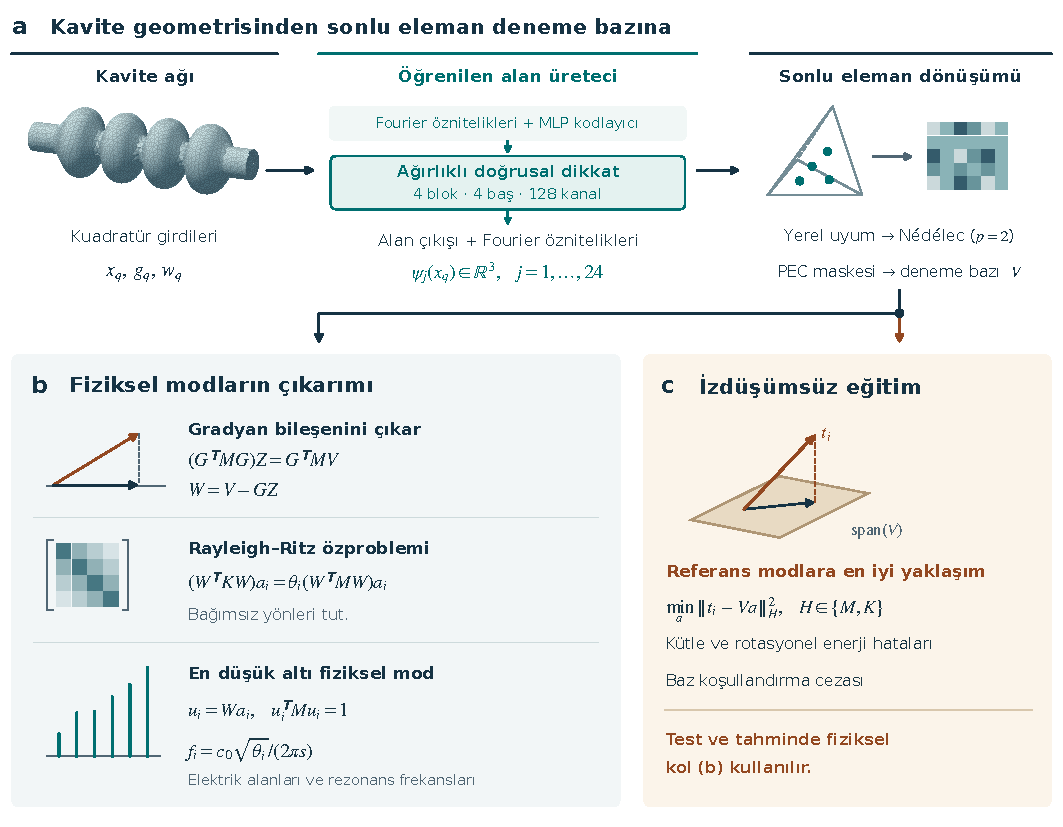
\includegraphics[width=\textwidth]{rf-model-tr.pdf}
  \caption{Üç boyutlu RF kavitelerinde rezonans modlarını tahmin eden sinir operatörü.
  (a) Ağ, her hacim kuadratür noktasının konumunu $x_q$, geometrik özniteliklerini $g_q$ ve normalize edilmiş integrasyon ağırlığını $w_q$ kullanır. Ağırlıklar doğrusal dikkat toplamına girer. Üretilen 24 vektör alanı eleman bazında polinomlarla yaklaştırılır ve ikinci derece Nédélec uzayına aktarılır. Mükemmel iletken (PEC) duvarda teğetsel serbestlik derecelerinin sıfırlanması deneme bazı $V$'yi verir.
  (b) Tahminde ayrık gradyan $G$ ve kütle matrisi $M$ ile gradyan bileşeni çıkarılır. Kalan uzayda, $K$ rotasyonel enerji matrisi olmak üzere, Rayleigh--Ritz çözümü yeterli sayısal rütbe varsa en düşük altı modun elektrik alanlarını ve frekanslarını verir. $c_0$ boşluktaki ışık hızı, $s$ geometriyi boyutsuzlaştıran uzunluk ölçeğidir. Spektrum çizimi temsilidir.
  (c) Gösterilen izdüşümsüz eğitim ayarında referans sonlu eleman modu $t_i$ için $V$ içinde kütle ve enerji ölçülerinde en iyi yaklaşım aranır. Eğitim ve doğrulamada bağıl artıklar bir baz koşullandırma terimiyle birlikte kullanılır.}
  \label{fig:rf-model-tr}
\end{figure*}
